%-------------------------------------------------------------------------------
%	PACKAGES AND THEMES
%-------------------------------------------------------------------------------

\documentclass{beamer}

\usetheme{focus} % Use the Focus theme supplied with the template
% Add option [numbering=none] to disable the footer progress bar
% Add option [numbering=fullbar] to show the footer progress bar as always full with a slide count

% Uncomment to enable the ice-blue theme
%\definecolor{main}{RGB}{92, 138, 168}
%\definecolor{background}{RGB}{240, 247, 255}

\usepackage{booktabs} % Required for better table rules
\usepackage{amsmath}
\usepackage{nccmath}
\usepackage{xcolor}

% set objects in itemize as triangles
\setbeamertemplate{itemize items}[triangle]

\newcommand{\indep}{\perp \!\!\! \perp}
\DeclareMathOperator*{\argmax}{arg\,max}

%-------------------------------------------------------------------------------
%	TITLE PAGE
%-------------------------------------------------------------------------------

\title{Does Money Buy Success?}

\subtitle{\large{Teams' Value and Match Outcomes in the Bundesliga}}

\author{Alec Eisenkolb, Chung Shun Man, \\Nicolas Greber, and Tim Hug} % Name
\institute{University of St. Gallen \\}

\date{26. May 2021} % Date

%-------------------------------------------------------------------------------
%	BEGIN DOCUMENT
%-------------------------------------------------------------------------------

\begin{document}

\begin{frame}

  \maketitle % Print the title page as the first slide

\end{frame}

% \begin{frame}
% \frametitle{Overview} % Table of contents slide
% \tableofcontents
% \end{frame}

%-------------------------------------------------------------------------------
%	PRESENTATION SLIDES
%-------------------------------------------------------------------------------

%-------------------------------------
%	DATA
%-------------------------------------

\begin{frame}
\frametitle{Outcome Variable}

\begin{figure}
	\centering
	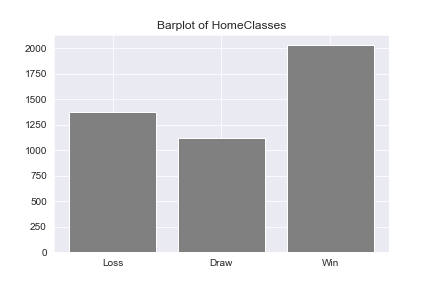
\includegraphics[scale=0.4]{img/histogram_of_HomeClassesKopie.png}
	\caption{Histogram of Match Outcomes}
\end{figure}

	\begin{columns}[T]
		\begin{column}{.5\textwidth}
			\begin{itemize}
				\item Match Outcomes from the Home team perspective
			\end{itemize}
		\end{column}

		\begin{column}{.5\textwidth}
			\begin{itemize}
				\item Unconditional probabilities indicate that Home team has a higher likelihood of winning
			\end{itemize}
		\end{column}
	\end{columns}

\end{frame}


\begin{frame}
\frametitle{Treatment Variable | 1}

\begin{figure}
	\centering
	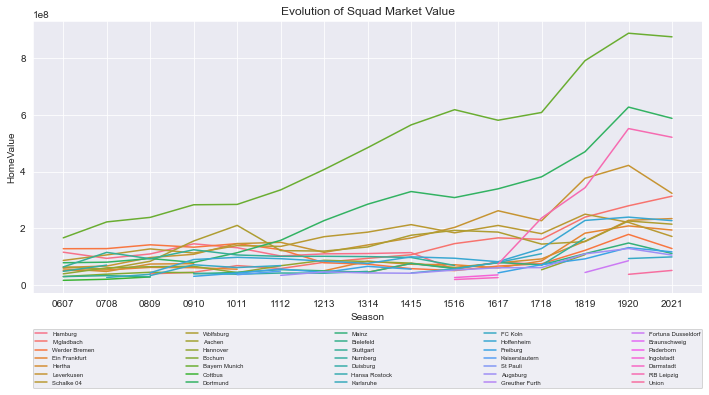
\includegraphics[scale=0.45]{img/MarkVal2Kopie.png}
	\caption{Histogram of Match Outcomes}
\end{figure}

\end{frame}


\begin{frame}
\frametitle{Treatment Variable | 2}

	\begin{columns}[T]
		\begin{column}{.4\textwidth}			
			\begin{table}[ht]
				\centering
				\scalebox{0.7}{
				\begin{tabular}{lll}
					\toprule
					{} & HomeHigherVal &   Obs \\
					HomeClasses &               &       \\
					\midrule
					Loss          &         0.334 &  1378 \\
					Draw           &         0.491 &  1117 \\
					Win           &          0.62 &  2032 \\
					\bottomrule
				\end{tabular}}
				\caption{Mean of treatment for match outcome}
			\end{table}
		\end{column}

		\begin{column}{.45\textwidth}
			\begin{itemize}
				\item Creating a dummy variable, indicating if Home team is more expensive 
				\item Indicate a positive trend between higher market value and likelihood of winning
			\end{itemize}
		\end{column}
	\end{columns}

\end{frame}


\begin{frame}
\frametitle{Covariates}

	\begin{columns}[T]
		\begin{column}{.48\textwidth}
			\textbf{Macro Variables}
			\begin{itemize}
				\item Diff in GDP, unemployment and TV revenue. 
			\end{itemize}				
			
			\textbf{Seasonal Dummies}				
			\begin{itemize}
				\item Dummy variables to control for each season, 06/07 - 19/20, with 20/21 being the base 								dummy. 
			\end{itemize}
		\end{column}
		
		\begin{column}{.48\textwidth}			
			\textbf{Team Stats}
			\begin{itemize}
				\item Age, Height, Champions, Relegated
			\end{itemize}
			
			\textbf{Match Stats}
			\begin{itemize}
				\item Shots on target, fouls, yellow/red cards, corners
				\item Attendance 
			\end{itemize}
		\end{column}
	\end{columns}

\begin{center}
	In total, 43 covariates, including the treatment variable. 
\end{center}

\end{frame}

%------------------------------------------------

%-------------------------------------
%	METHODS
%-------------------------------------

\begin{frame}
	\frametitle{Estimators | 1}

	\begin{columns}[T]
		\begin{column}{.48\textwidth}
			\textbf{Ordinal Logistic Regression}

			\begin{itemize}
				\item Parametric estimator
				\item Latent linear model
				\item Assume logistic distribution
				\item Min. maximum margin loss function
				\begin{itemize}
					\item Gradient descent
					\item SciPy optimizer
				\end{itemize}
			\end{itemize}

		\end{column}

		\begin{column}{.48\textwidth}
			\textbf{Ordered Random Forest}

			\begin{itemize}
				\item Non-parametric estimator
				\item Based on binary forest regression
				\item No distributional assumption required
				\item Min. mean squared error
			\end{itemize}

		\end{column}
	\end{columns}

\end{frame}

%------------------------------------------------

\begin{frame}
	\frametitle{Estimators | 2}

	Two different models...

	\begin{itemize}
		\item Parametric vs. non-parametric estimator
		\item Distributional assumption
	\end{itemize}

	\vfill

	\begin{block}{Conclusion}
		Model specification is correct and distributional assumption holds\\
		$\Rightarrow$ logit model may be the more efficient estimator
	\end{block}

\end{frame}

% \begin{frame}
% \frametitle{Logistic Regression}
%
% \begin{columns}[T]
%   \begin{column}{.48\textwidth}
%     \begin{equation*}
%       Y^{*} = X\beta + U, \quad U | X = x \sim F(0, \sigma^2)
%     \end{equation*}
%
%     \begin{equation*}
%       \alpha_1 < \alpha_2
%     \end{equation*}
%
%     \begin{itemize}
%       \item Objective according to a maximum margin loss
%     \end{itemize}
%
%     \begin{equation*}
%       x^{(k + 1)} = x^{(k)} - \alpha \cdot \nabla f(x^{(k)})
%     \end{equation*}
%
%     \begin{itemize}
%       \item Gradient descent as optimization algorithm
%     \end{itemize}
%
%   \end{column}
%
%   \begin{column}{.38\textwidth}
%     \begin{figure}
%       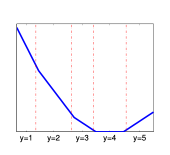
\includegraphics[width=0.9\textwidth]{img/allthreshold_loss.png}
%       \caption{All-threshold based loss}
%     \end{figure}
%   \end{column}
% \end{columns}
%
% \end{frame}

%------------------------------------------------

% \begin{frame}
% \frametitle{Ordered Forest}
%
% \begin{columns}[T]
%   \begin{column}{.68\textwidth}
%    \begin{itemize}
%    \item An ordered forest is based on binary forest regression
%    \item A forest is built on bootstrapped sample trees
%    \item Predict the class 1 dummy and cumulative class 1 and 2 dummy
%    \item Difference the culmulative probabailities to get the isolated probabilities
%    \end{itemize}
%    \end{column}
%
%   \begin{column}{.44\textwidth}
%     		\begin{equation*}
%    		\text{Cul} P_{m,i} = \begin
% 		{bmatrix}P_{1,1}\quad P_{(1,2),1}\\
% 		P_{1,2}\quad P_{(1,2),2}\\
% 		\vdots\quad \vdots\\
% 		P_{1,n}\quad P_{(1,2),n}\\
% 		\end{bmatrix}
% 	  \end{equation*}
% 	  \begin{equation*}
%   		\text{Iso} P_{m,i} = \begin{bmatrix}
% 		P_{1,1} & P_{2,1} & P_{3,1}\\
% 		P_{1,2} & P_{2,2} & P_{3,2}\\
% 		\vdots & \vdots & \vdots\\
% 		P_{1,n} & P_{2,n} & P_{3,n}\\
% 		\end{bmatrix}
% 	  \end{equation*}
% 	  \begin{tiny}
% 	  where m, i = class and observation number
% 	  \end{tiny}
%
%   \end{column}
%
% \end{columns}
%
%
% \end{frame}


%------------------------------------------------

%-------------------------------------
%	RESULTS
%-------------------------------------

\begin{frame}
\frametitle{Results}


\begin{columns}
  \begin{column}{.50\textwidth}
   \begin{itemize}
   \setlength\itemsep{1em}
   \item Mean marginal effects are chosen in the design
   \item Both models are credible. 
   \item A more valuable home team should expect 0.212 or 0.165 more points
   \end{itemize}
   \end{column}


\begin{column}{0.50 \textwidth}
\begin{table}[ht]
\centering
	\begin{tabular}{lrr}
	\toprule
	{} &   OLogit &   ORF  \\
	\midrule
	0 point & -0.063 & -0.061\\
	1 point    & -0.011 & 0.09\\
	3 points & 0.074 & 0.052\\
	\bottomrule
	\end{tabular}
	\caption{ATE of higher home value}
	\label{tab:MeanMarg}
\end{table}

\begin{table}[ht]
\centering
	\begin{tabular}{lll}
	\toprule
	{}   & OLogit & ORF \\
	\midrule
	Extra points &  0.212 &  0.165 \\
	\bottomrule
	\end{tabular}
	\caption{Extra points}
	\label{tab:numpoints}
\end{table}
\end{column}
\end{columns}

\end{frame}

%------------------------------------------------
%------------------------------------------------

\begin{frame}
\frametitle{Robustness check}

\textbf{Test 1}: Evolution of ATEs over the seasons

\begin{columns}
  \begin{column}{0.5\textwidth}
    \begin{figure}
      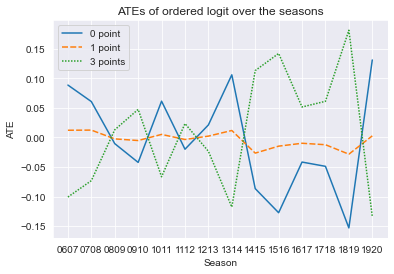
\includegraphics[width=1\textwidth]{img/ATEs_logit.png}
    \end{figure}
   \end{column}

   \begin{column}{0.5\textwidth}
    \begin{figure}
      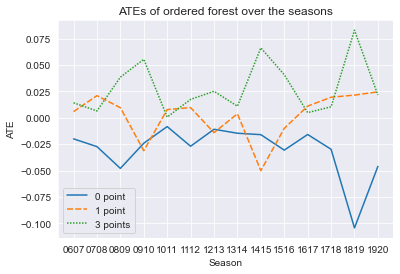
\includegraphics[width=1\textwidth]{img/ATEs_orf.png}
    \end{figure}
  \end{column}
\end{columns}
\
\\
\textbf{Test 2}: Removal of outliers (Bayern Munich and Dortmund)
\begin{itemize}
\item The marginal effects drop. A more expensive home team should expect between 0.16 and 0.11.
\end{itemize}

\end{frame}




\begin{frame}
\frametitle{Prediction Performance}

\begin{columns}[T]
	\begin{column}{.4\textwidth}			
		\begin{table}[ht]
			\centering
			\begin{tabular}{lrr} \toprule {}
	  			&     $MSE \footnote[frame]{$MSE = \frac{1}{N} \sum_{i = 0}^N \sum_{j=1}^J (I(Y_i = j) - \hat{P}[Y_i = j \mid X_i = x])^2$ \vspace{1mm}}$  & $CA$ \\
	  			\midrule
				OLogit  &  1.025  & 0.487 \\
				ORF &     0.586  & 0.527 \\  \midrule
				\bottomrule
			\end{tabular}
			\caption{Prediction performance for both estimators.}
			\label{tab:predictions}
		\end{table}		
	\end{column}

	\begin{column}{.45\textwidth}
	\vspace{1cm}
		\begin{itemize}
			\item ORF performs better in terms of MSE and CA		
			\item Logit model has troubles estimating class 1 (draw)
		\end{itemize}
	\end{column}
\end{columns}

\end{frame}

\begin{frame}
\frametitle{Discussion}

\textbf{Identifying Assumptions:}
\begin{itemize}
\item Conditional independence
\begin{itemize}
\item Control for the most important confounders
\item In line with current literature
\end{itemize}

\item Common support
\begin{itemize}
\item Given by the structure of the data
\end{itemize}

\item Exogeneity of confounders
\begin{itemize}
\item Market value could influence match related variables
\end{itemize}

\item Stable unit treatment value assumption

\end{itemize}
\end{frame}


%------------------------------------------------



%------------------------------------------------

\begin{frame}
\frametitle{Summary}

\begin{itemize}
\item Overview of the data
\item Estimation with Ordered Logit Regression and Ordered Random Forest
\item Result: A more valuable home team can expect \\ 0.212 (Ordered Logit) or 0.165 (ORF) more points.
\item Causal effect may be biased towards zero because exogeneity assumption may not hold. 
\end{itemize}

\end{frame}

\end{document}
